This Chapter summarises the structure of the information necessary to define
a PSHA input model to be used with the \glsdesc{acr:oqe}.

Input data for probabilistic based seismic hazard analysis (Classical, Event
based, Disaggregation, and UHS) are organised into:

\begin{itemize}

	\item A general configuration file.

    \item A file describing the Seismic Source System, that is the set of
	initial source models and associated epistemic uncertainties needed to
	model the seismic activity in the region of interest.

    \item A file describing the Ground Motion System, that is the set of
	ground motion prediction equations, per tectonic region type, needed to
	model the ground motion shaking in the region of interest.

\end{itemize}

Figure~\ref{fig:psha_input} summarises the structure of a PSHA input model
for the \glsdesc{acr:oqe} and the relationships between the different files.

\begin{figure}[!ht]
\centering
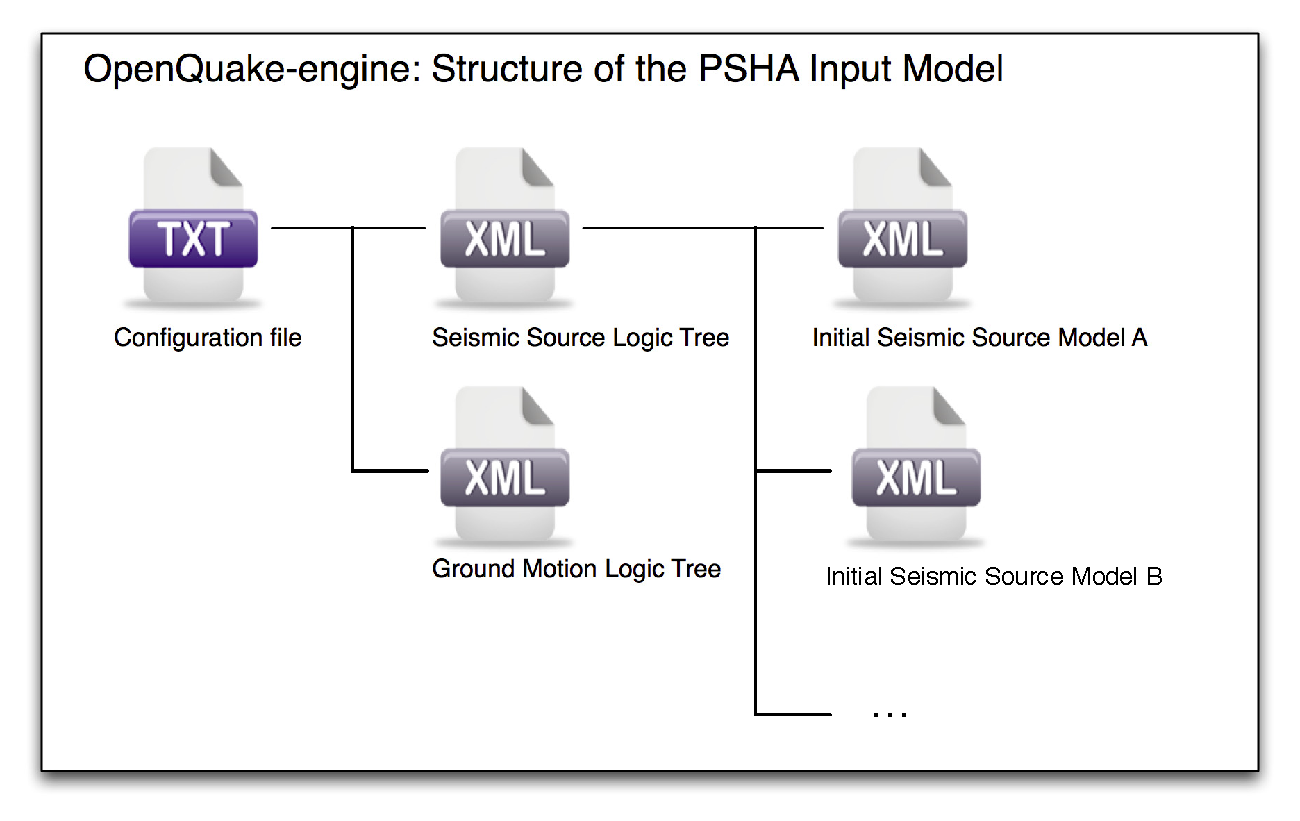
\includegraphics[width=14cm]{figures/hazard/psha_input_structure.pdf}
\caption{PSHA Input Model structure}
\label{fig:psha_input}
\end{figure}


\section{Defining Logic Trees}
The main components of a logic tree structure in the OpenQuake engine are 
the following:
\begin{description}
    \item[branch]: the simplest component of a logic tree structure. 
    A branch represents a possible interpretation/value assignment of 
    a type of uncertainty. It is fully described by the tuple 
    (parameter/model, weight).
    
    \item[branching set]: a key component in the logic tree structure 
    used by the \gls{acr:oqe}. It groups a set of branches i.e. 
    alternative interpretations of a parameter or a model. Each branching
    set is defined by:
    \begin{itemize}
        \item An ID 
        \item An uncertainty type (for a comprehensive list of the types of 
        uncertainty currently supported see Section )
        \item One or more branches
    \end{itemize}
    
    This set of uncertainties can be applied to the whole initial 
    seismic source input model or just to a subset of seismic source
    data. The sum of the weights/probabilities assigned to the set 
    of branches. 

    \item[branching level]: the largest container. It's not used in 
    modelling uncertainty, but it's useful in maintaining a logic and an 
    order in the structure of the tree.
\end{description}

Below we provide a simple schema illustrating the skeleton of the 
\gls{acr:oqe} logic tree:
\begin{Verbatim}[frame=single, commandchars=\\\{\}, fontsize=\small]
\textcolor{green}{<logicTreeBranchingLevel branchingLevelID=ID>}
    \textcolor{blue}{<logicTreeBranchSet branchSetID=ID}
            \textcolor{blue}{uncertaintyType=TYPE>}
        \textcolor{magenta}{<logicTreeBranch>}
            \textcolor{cyan}{<uncertaintyModel>VALUE</uncertaintyModel>}
            \textcolor{cyan}{<uncertaintyWeight>WEIGHT</uncertaintyWeight>}
        \textcolor{magenta}{</logicTreeBranch>}
    \textcolor{blue}{</logicTreeBranchSet>}
\textcolor{green}{</logicTreeBranchingLevel>}
\end{Verbatim}

A schematic representation of these three objects is provided in Figure 
\ref{glts}. A branching level identifies the position in a tree where
branching occurs while a branch set identifies a collection of branches 
(i.e. individual branches) whose weights sum to 1.\\
%
\begin{figure}[!h]
\centering
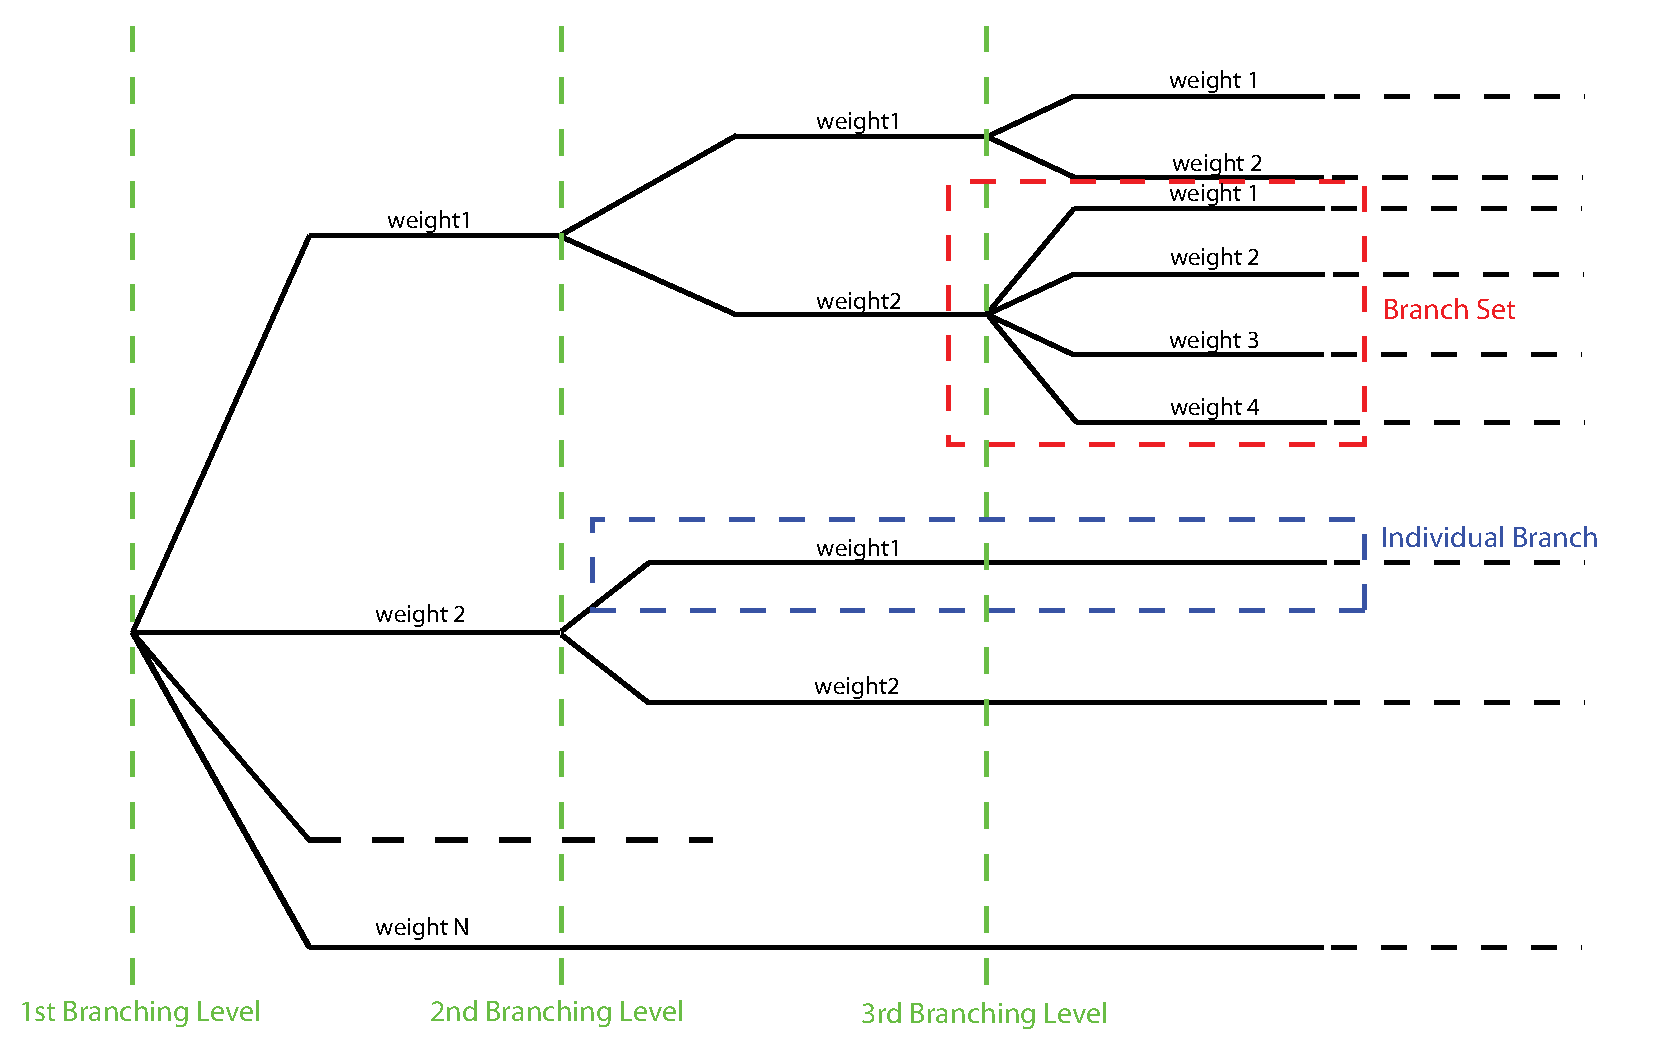
\includegraphics[width=15cm]{./figures/hazard/GenericLogicTreeStructure.eps}
\caption{Generic Logic Tree structure as described in terms of branching 
levels, branch sets, and individual branches.}
\label{glts}
\end{figure}
%
In the NRML schema, a logic tree structure is defined through the 
\Verb+logicTree+ element: 
%
\begin{Verbatim}[frame=single, commandchars=\\\{\}]
<\textcolor{red}{logicTree} logicTreeID="ID">
...
</\textcolor{red}{logicTree}>
\end{Verbatim}
%
A \Verb+logicTree+ contains as a sequence of \Verb+logicTreeBranchingLevel+ 
elements. The position in the sequence specifies in which level of the tree 
the branching level is located. That is, the first 
\texttt{logicTreeBranchingLevel} element in the sequence represents the first 
level in the tree, the second element the second level in the tree, and so on.
%
\begin{Verbatim}[frame=single, commandchars=\\\{\}]
<\textcolor{red}{logicTree} logicTreeID="ID">
	<\textcolor{green}{logicTreeBranchingLevel} branchingLevelID="ID_1">
		...
	</\textcolor{green}{logicTreeBranchingLevel}>
	<\textcolor{green}{logicTreeBranchingLevel} branchingLevelID="ID_2">
		...
	</\textcolor{green}{logicTreeBranchingLevel}>
	....
	<\textcolor{green}{logicTreeBranchingLevel} branchingLevelID="ID_N">
		...
	</\textcolor{green}{logicTreeBranchingLevel}>
</\textcolor{red}{logicTree}>
\end{Verbatim}
No restrictions are present on the number of tree levels that can 
be defined.

A \Verb+logicTreeBranchingLevel+ is defined as a sequence of 
\Verb+logicTreeBranchSet+ elements. Each \Verb+logicTreeBranchSet+ 
defines a particular epistemic uncertainty inside a branching level. 

A branch set has two required attributes (\Verb+branchSetID+ and 
\Verb+uncertaintyType+ (defining the type of epistemic uncertainty 
the branch set is defining))
\begin{Verbatim}[frame=single, commandchars=\\\{\}]
<\textcolor{red}{logicTree} logicTreeID="ID">
...
	<\textcolor{green}{logicTreeBranchingLevel} branchingLevelID="ID_#">
		<\textcolor{blue}{logicTreeBranchSet} branchSetID="ID_1"
			uncertaintyType="UNCERTAINTY_TYPE">
			...
		</\textcolor{blue}{logicTreeBranchSet}>
		<\textcolor{blue}{logicTreeBranchSet} branchSetID="ID_2"
			uncertaintyType="UNCERTAINTY_TYPE">
			...
		</\textcolor{blue}{logicTreeBranchSet}>
		...
		<\textcolor{blue}{logicTreeBranchSet} branchSetID="ID_N"
			uncertaintyType="UNCERTAINTY_TYPE">
			...
		</\textcolor{blue}{logicTreeBranchSet}>
	</\textcolor{green}{logicTreeBranchingLevel}>
...
</\textcolor{red}{logicTree}>
\end{Verbatim}
Possible values for the \Verb+uncertaintyType+ attribute are:
\begin{itemize}
\item \Verb+gmpeModel+: identifying epistemic uncertainties on ground 
motion prediction equations
\item \Verb+sourceModel+: identifying epistemic uncertainties on source models
\item \Verb+maxMagGRRelative+: identifying epistemic uncertainties 
(relative: that is increments) to be added (or subtracted, depending on 
the sign of the increment) to the 
Guten\-berg-Richter maximum magnitude value.
\item \Verb+bGRRelative+: identifying epistemic uncertainties (relative)
to be applied to the Guten\-berg-Richter b value.
\item \Verb+abGRAbsolute+:identifying epistemic uncertainties (absolute: 
that is new values used to replace original values) on the Guten\-berg-Richter
a and b values.
\item \Verb+maxMagGRAbsolute+: identifying epistemic uncertainties 
(absolute) on the Guten\-berg-Richter maximum magnitude.
\end{itemize}
No restrictions are given on the number of branch sets that can be defined 
inside a branching level.

A \Verb+branchSet+ is defined as a sequence of \Verb+logicTreeBranch+ 
elements, each specified by an \Verb+uncertaintyModel+ element (a string 
identifying an uncertainty mod\-el; the content of the string varies with
the uncertaintyType attribute value of the branchSet element) and the
uncertaintyWeight element (specifying the probability/weight associated 
to the uncertaintyModel):
\begin{Verbatim}[frame=single, commandchars=\\\{\}]
<\textcolor{red}{logicTree} logicTreeID="ID">
...
	<\textcolor{green}{logicTreeBranchingLevel} branchingLevelID="ID_#">
		...
		<\textcolor{blue}{logicTreeBranchSet} branchSetID="ID_#"
				uncertaintyType="UNCERTAINTY_TYPE">
			<\textcolor{magenta}{logicTreeBranch} branchID="ID_1">
				<uncertaintyModel>
				UNCERTAINTY_MODEL
				</uncertaintyModel>
				<uncertaintyWeight>
				UNCERTAINTY_WEIGHT
				</uncertaintyWeight>
			</\textcolor{magenta}{logicTreeBranch}>
			...
			<\textcolor{magenta}{logicTreeBranch} branchID="ID_N">
				<uncertaintyModel>
				UNCERTAINTY_MODEL
				</uncertaintyModel>
				<uncertaintyWeight>
				UNCERTAINTY_WEIGHT
				</uncertaintyWeight>
			</\textcolor{magenta}{logicTreeBranch}>
		</\textcolor{blue}{logicTreeBranchSet}>
		...
	</\textcolor{green}{logicTreeBranchingLevel}>
...
</\textcolor{red}{logicTree}>
\end{Verbatim}
Depending on the \Verb+uncertaintyType+ the content of the 
\Verb+<uncertaintyModel>+ element changes:
\begin{itemize}
\item if \Verb+uncertaintyType="gmpeModel"+, the uncertainty model 
contains the name of a ground motion prediction equation (a list of 
available GMPEs are given in appendix A), e.g.:
\begin{Verbatim}[frame=single, commandchars=\\\{\}]
<uncertaintyModel>GMPE_NAME</uncertaintyModel>
\end{Verbatim}
\item if \Verb+uncertaintyType="sourceModel"+, the uncertainty model contains 
the paths to a source model file, e.g.:
\begin{Verbatim}[frame=single, commandchars=\\\{\}]
<uncertaintyModel>SOURCE_MODEL_FILE_PATH</uncertaintyModel>
\end{Verbatim}
\item if \Verb+uncertaintyType="maxMagGRRelative"+, the uncertainty model 
contains the increment to be added (or subtracted, depending on the sign) 
to the Guten\-berg-Richter maximum magnitude:
\begin{Verbatim}[frame=single, commandchars=\\\{\}, samepage=true]
<uncertaintyModel>MAX_MAGNITUDE_INCREMENT</uncertaintyModel>
\end{Verbatim}
\item if \Verb+uncertaintyType="bGRRelative"+, the uncertainty model 
contains the increment to be added (or subtracted, depending on the 
sign) to the Guten\-berg-Richter b value:
\begin{Verbatim}[frame=single, commandchars=\\\{\}, samepage=true]
<uncertaintyModel>B_VALUE_INCREMENT</uncertaintyModel>
\end{Verbatim}
\item if \Verb+uncertaintyType="abGRAbsolute"+, the uncertainty model 
contains one (if the uncertainty apply to a source with only one 
Guten\-berg-Richter magnitude frequency distribution) or more (if the 
source has more than one magnitude frequency distributions) a and b pairs:
\begin{Verbatim}[frame=single, commandchars=\\\{\}, samepage=true]
<uncertaintyModel>
A_VALUE_1 B_VALUE_1
 ... 
A_VALUE_N B_VALUE_N
</uncertaintyModel>
\end{Verbatim}
    \item if \Verb+uncertaintyType="maxMagGRAbsolute"+, the uncertainty 
    model contains one or more (depending on the number of magnitude 
    frequency distributions in the source) Guten\-berg-Richter maximum 
    magnitude values:
%
\begin{Verbatim}[frame=single, commandchars=\\\{\}, samepage=true]
<uncertaintyModel>
MAX_MAGNITUDE_1
 ... 
MAX_MAGNITUDE_N
</uncertaintyModel>
\end{Verbatim}
\end{itemize}
%
No restrictions are given on the number of \Verb+logicTreeBranch+ elements 
that can be defined in a \Verb+logicTreeBranchSet+, as long as the uncertainty 
weights sum to 1.0.

The \Verb+logicTreeBranchSet+ element offers also a number of optional 
attributes allowing for complex tree definitions:
\begin{itemize}
    \item \Verb+applyToBranches+: specifies to which \Verb+logicTreeBranch+ 
    elements (one or more), in the previous branching level, the branch set 
    is linked to. The linking is established by defining the IDs of the 
    branches to link to:
\begin{Verbatim}[frame=single, commandchars=\\\{\}, samepage=true]
applyToBranches="branchID1 branchID2 .... branchIDN"
\end{Verbatim}
    The default is the keyword ALL, which means that a branch set is by default 
    linked to all branches in the previous branching level. By specifying one or 
    more branches to which the branch set links to, non-symmetric logic trees 
    can be defined.
    \item \Verb+applyToSources+: specifies to which source in a source model 
        the uncertainty applies to. Sources are specified in terms of their IDs:
\begin{Verbatim}[frame=single, commandchars=\\\{\}, samepage=true]
applyToSources="srcID1 srcID2 .... srcIDN"
\end{Verbatim}
    \item \Verb+applyToSourceType+: specifies to which source type the 
    uncertainty applies to.  Only one source typology can be defined 
    (\Verb+area+, \Verb+point+, \texttt{simple\-Fault}, 
	\Verb+complexFault+), e.g.:
\begin{Verbatim}[frame=single, commandchars=\\\{\}, samepage=true]
applyToSources="area"
\end{Verbatim}
    \item \Verb+applyToTectonicRegionType+: specifies to which tectonic 
    region type the uncertainty applies to. Only one tectonic region type 
    can be defined (\texttt{Ac\-tive} \texttt{Shallow Crust}, 
    \Verb+Stable Shallow Crust+, \Verb+Subduction Interface+, 
    \texttt{Sub\-duc\-tion} \texttt{IntraSlab}, \texttt{Volcanic}), e.g.:
\begin{Verbatim}[frame=single, commandchars=\\\{\}]
applyToTectonicRegionType="Active Shallow Crust"
\end{Verbatim}
\end{itemize}

\label{sec:hazard_logic_trees}

\section{The Seismic Source System}
The Seismic Source System contains the model (or the models) describing
position, geometry and activity of seismic sources of engineering importance
for a set of sites as well as the possible epistemic uncertainties to be
incorporated into the calculation of seismic hazard.



\subsection{The Seismic Source Logic Tree}

The structure of the Seismic Source Logic Tree consists of at least one
\gls{branchinglevel}. This branching level is the one used to define the
\gls{initialseismicsourceinputmodel} (or a number of initial seismic source
models, see Figure~\ref{fig:psha_input}).

The example provided below shows the simplest Seismic Source Logic Tree
structure that can be defined in a \gls{pshainputmodel} for \gls{acr:oqe}. It's a logic tree with just one branching level containing one \gls{branchset} with one branch used to define the initial seismic source model (its weight will be equal to one). 

\begin{minted}[firstline=1,firstnumber=1,fontsize=\footnotesize,frame=single,bgcolor=lightgray]{xml}
<?xml version="1.0" encoding="UTF-8"?>
<nrml xmlns:gml="http://www.opengis.net/gml"
      xmlns="http://openquake.org/xmlns/nrml/0.5">
    <logicTree logicTreeID="lt1">
        <logicTreeBranchingLevel branchingLevelID="bl1">
            <logicTreeBranchSet uncertaintyType="sourceModel"
                                branchSetID="bs1">
                <logicTreeBranch branchID="b1">
                    <uncertaintyModel>seismic_source_model.xml
                    </uncertaintyModel>
                    <uncertaintyWeight>1.0</uncertaintyWeight>
                </logicTreeBranch>
            </logicTreeBranchSet>
        </logicTreeBranchingLevel>
    </logicTree>
</nrml>
\end{minted}

%\begin{Verbatim}[frame=single, commandchars=\\\{\}, fontsize=\small,
    firstnumber=1, numbers=left, numbersep=2pt]
<?xml version="1.0" encoding="UTF-8"?>
<nrml xmlns:gml="http://www.opengis.net/gml"
      xmlns="http://openquake.org/xmlns/nrml/0.5">
    <logicTree logicTreeID="lt1">
        <logicTreeBranchingLevel branchingLevelID="bl1">
            <logicTreeBranchSet uncertaintyType="sourceModel"
                                branchSetID="bs1">
                <logicTreeBranch branchID="b1">
                    <uncertaintyModel>seismic_source_model.xml
                    </uncertaintyModel>
                    <uncertaintyWeight>1.0</uncertaintyWeight>
                </logicTreeBranch>
            </logicTreeBranchSet>
        </logicTreeBranchingLevel>
    </logicTree>
</nrml>
\end{Verbatim}

The optional branching levels will contain rules that modify parameters of the sources in the initial seismic source model.

For example, if the epistemic uncertainties to be considered are source
geometry and maximum magnitude, the modeller can create a logic tree structure with three initial seismic source models (each one exploring a different definition of the geometry of sources) and one branching level accounting for the epistemic uncertainty on the maximum magnitude.

Below we provide an example of such logic tree structure. Note that the uncertainty on the maximum magnitude is specified in terms of relative increments with respect to the initial maximum magnitude defined for each source in the initial seismic source models.

\inputminted[firstline=1,firstnumber=1,fontsize=\footnotesize,frame=single,linenos,bgcolor=lightgray]{xml}{oqum/hazard/verbatim/input_sslt_simple_lt.xml}
\captionof{listing}{Example source model logic tree structure\label{lst:example_source_model_logic_tree}}

%\begin{Verbatim}[frame=single, commandchars=\\\{\}, fontsize=\small,
    firstnumber=1, numbers=left, numbersep=2pt]
<?xml version="1.0" encoding="UTF-8"?>
<nrml xmlns:gml="http://www.opengis.net/gml"
      xmlns="http://openquake.org/xmlns/nrml/0.5">
    <logicTree logicTreeID="lt1">

        <logicTreeBranchingLevel branchingLevelID="bl1">
            <logicTreeBranchSet uncertaintyType="sourceModel"
                                branchSetID="bs1">
                <logicTreeBranch branchID="b1">
                    <uncertaintyModel>seismic_source_model_A.xml
                    </uncertaintyModel>
                    <uncertaintyWeight>0.2</uncertaintyWeight>
                </logicTreeBranch>
                <logicTreeBranch branchID="b2">
                    <uncertaintyModel>seismic_source_model_B.xml
                    </uncertaintyModel>
                    <uncertaintyWeight>0.3</uncertaintyWeight>
                </logicTreeBranch>
                <logicTreeBranch branchID="b3">
                    <uncertaintyModel>seismic_source_model_C.xml
                    </uncertaintyModel>
                    <uncertaintyWeight>0.5</uncertaintyWeight>
                </logicTreeBranch>
            </logicTreeBranchSet>
        </logicTreeBranchingLevel>

        <logicTreeBranchingLevel branchingLevelID="bl2">
            <logicTreeBranchSet branchSetID="bs21" 
                    uncertaintyType="maxMagGRRelative">
                <logicTreeBranch branchID="b211">
                    <uncertaintyModel>+0.0</uncertaintyModel>
                    <uncertaintyWeight>0.6</uncertaintyWeight>
                </logicTreeBranch>
                <logicTreeBranch branchID="b212">
                    <uncertaintyModel>+0.5</uncertaintyModel>
                    <uncertaintyWeight>0.4</uncertaintyWeight>
                </logicTreeBranch>
            </logicTreeBranchSet>
        </logicTreeBranchingLevel>

    </logicTree>
</nrml>
\end{Verbatim}

\subsection{The Seismic Source Model}
\index{Input!Configuration file}

The structure of the xml file representing the seismic source model
corresponds to a list of sources, each one modelled using one out of the five
typologies currently supported. Below we provide a schematic example of a
seismic source model:

\begin{minted}[firstline=1,firstnumber=1,fontsize=\footnotesize,frame=single,bgcolor=lightgray]{xml}
< sourceModel  gml:id="ID">
	...
	< areaSource  gml:id="SOURCE_ID">
		<gml:name>SOURCE_NAME</gml:name>
		<tectonicRegion>TECT_REGION_TYPE</tectonicRegion>
		...
	</ areaSource >
	...
	< pointSource  gml:id="SOURCE_ID">
		<gml:name>SOURCE_NAME</gml:name>
		<tectonicRegion>TECT_REGION_TYPE</tectonicRegion>
		...
	</ pointSource >
	...
	< simpleFaultSource  gml:id="SOURCE_ID">
		<gml:name>SOURCE_NAME</gml:name>
		<tectonicRegion>TECT_REGION_TYPE</tectonicRegion>
		...
	</ simpleFaultSource >
	...
	< complexFaultSource  gml:id="SOURCE_ID">
		<gml:name>SOURCE_NAME</gml:name>
		<tectonicRegion>TECT_REGION_TYPE</tectonicRegion>
		...
	</ complexFaultSource >
	...
</ sourceModel >
\end{minted}

%\begin{Verbatim}[frame=single, commandchars=\\\{\}, fontsize=\small]
<\textcolor{red}{sourceModel} gml:id="ID">
	...
	<\textcolor{green}{areaSource} gml:id="SOURCE_ID">
		<gml:name>SOURCE_NAME</gml:name>
		<tectonicRegion>TECT_REGION_TYPE</tectonicRegion>
		...
	</\textcolor{green}{areaSource}>
	...
	<\textcolor{green}{pointSource} gml:id="SOURCE_ID">
		<gml:name>SOURCE_NAME</gml:name>
		<tectonicRegion>TECT_REGION_TYPE</tectonicRegion>
		...
	</\textcolor{green}{pointSource}>
	...
	<\textcolor{green}{simpleFaultSource} gml:id="SOURCE_ID">
		<gml:name>SOURCE_NAME</gml:name>
		<tectonicRegion>TECT_REGION_TYPE</tectonicRegion>
		...
	</\textcolor{green}{simpleFaultSource}>
	...
	<\textcolor{green}{complexFaultSource} gml:id="SOURCE_ID">
		<gml:name>SOURCE_NAME</gml:name>
		<tectonicRegion>TECT_REGION_TYPE</tectonicRegion>
		...
	</\textcolor{green}{complexFaultSource}>
	...
</\textcolor{red}{sourceModel}>
\end{Verbatim}

\label{sec:seismic_source_system}

\section{The Ground Motion System}
\index{Input!Ground motion system}
\label{sec:ground_motion_system}
The Ground Motion System defines the models and the possible epistemic
uncertainties related to ground motion modelling to be incorporated into the
calculation.

\subsection{The Ground Motion Logic Tree}
\index{Input!Ground motion logic tree}
\label{subsec:gmlt}

The structure of the \gls{groundmotionlogictree} consists of a list of ground
motion prediction equations for each tectonic region used to characterise the
sources in the PSHA input model.

The example below shows a simple \gls{groundmotionlogictree}. This logic tree
assumes that all the sources in the PSHA input model belong to ``Active
Shallow Crust'' and uses for calculation the \citet{chiou2008}
\gls{acr:gmpe}.

\begin{Verbatim}[frame=single, commandchars=\\\{\}, fontsize=\small,
    firstnumber=1, numbers=left, numbersep=2pt]
<?xml version="1.0" encoding="UTF-8"?>
<nrml xmlns:gml="http://www.opengis.net/gml"
      xmlns="http://openquake.org/xmlns/nrml/0.5">
    <logicTree logicTreeID='lt1'>
        <logicTreeBranchingLevel branchingLevelID="bl1">
            <logicTreeBranchSet uncertaintyType="gmpeModel"
                    branchSetID="bs1"
                    applyToTectonicRegionType="Active Shallow Crust">

                <logicTreeBranch branchID="b1">
                    <uncertaintyModel>
                    ChiouYoungs2008
                    </uncertaintyModel>
                    <uncertaintyWeight>1.0</uncertaintyWeight>
                </logicTreeBranch>

            </logicTreeBranchSet>
        </logicTreeBranchingLevel>
    </logicTree>
</nrml>
\end{Verbatim}


\section{Configuration file}
\index{Input!Configuration file!Hazard}
\label{sec:hazard_configuration_file}
The configuration file is the primary file controlling both the definition of
the input model as well as parameters governing the calculation. We illustrate
in the following different examples of the configuration file addressing
different typologies of seismic hazard calculation.


\subsection[Classical PSHA]{Classical PSHA}
\label{subsec:config_classical_psha}
In the following we describe the overall structure and the most typical
parameters of a configuration file to be used for the computation of a
seismic hazard map using a classical PSHA methodology.


\textbf{Calculation type and model info}

\begin{minted}[firstline=1,linenos=true,firstnumber=1,fontsize=\footnotesize,frame=single,bgcolor=lightgray]{ini}
[general]
description = A demo OpenQuake-engine .ini file for classical PSHA
calculation_mode = classical
random_seed = 1024
\end{minted}

In this section the user specifies the following parameters:

\begin{itemize}

    \item \texttt{description}: a parameter that can be used to designate
    the model

    \item \texttt{calculation\_mode}: it is used to set the kind of
    calculation. In this case it corresponds to \texttt{classical}.
    Alternative options for the calculation\_mode are described later in this
    manual.

    \item \texttt{random\_seed}: is used to control the random generator
    so that when Monte Carlo procedures are used calculations are
    replicable (if the same \texttt{random\_seed} is used you get exactly
    the same results).

\end{itemize}

\textbf{Geometry of the area (or the sites) where hazard is computed}

This section is used to specify where the hazard will be computed. Two
options are available:

The first ooption is to define a polygon (usually a rectangle) and a distance
(in km) to be used to discretize the  polygon area. The polygon is defined by
a list of longitude-latitude tuples.

An example is provided below:

\begin{minted}[firstline=1,linenos=true,firstnumber=5,fontsize=\footnotesize,frame=single,bgcolor=lightgray]{ini}
[geometry]
region = 10.0 43.0, 12.0 43.0, 12.0 46.0, 10.0 46.0
region_grid_spacing = 10.0
\end{minted}

The second option allows the definition of a number of sites where the hazard
will be computed. An example is provided below:

\begin{minted}[firstline=1,linenos=true,firstnumber=8,fontsize=\footnotesize,frame=single,bgcolor=lightgray]{ini}
[geometry]
sites = 10.0 43.0, 12.0 43.0, 12.0 46.0, 10.0 46.0
\end{minted}

If the list of sites is too long the user can specify the name of a csv file
as shown below:

\begin{minted}[firstline=1,linenos=true,firstnumber=10,fontsize=\footnotesize,frame=single,bgcolor=lightgray]{ini}
[geometry]
sites_csv = <name_of_the_csv_file>
\end{minted}

The format of the csv file containing the list of sites is a sequence of
points (one per row) specified in terms of the longitude, latitude tuple. An
example is provided below:

\begin{minted}[firstline=1,linenos=false,firstnumber=10,fontsize=\footnotesize,frame=single,bgcolor=lightgray]{text}
179.0,90.0
178.0,89.0
177.0,88.0
\end{minted}

\textbf{Logic tree sampling}

The \gls{acr:oqe} provides two options for processing the whole logic tree
structure. The first option uses Montecarlo sampling; the user in this case
specifies a number of realizations.

In the second option all the possible realizations are created. Below we
provide an example for the latter option. In this case we set the
\texttt{number\-\_of\-\_logic\_tree\_samples} to 0. \gls{acr:oqe} will perform
a complete enumeration of all  the possible paths from the roots to the leaves
of the logic tree  structure.

\begin{minted}[firstline=1,linenos=true,firstnumber=12,fontsize=\footnotesize,frame=single,bgcolor=lightgray]{ini}
[logic_tree]
number_of_logic_tree_samples = 0
\end{minted}

If the seismic source logic tree and the ground motion logic tree do not
contain epistemic uncertainties the engine will create a single PSHA input.

\textbf{Generation of the earthquake rupture forecast}

\begin{minted}[firstline=1,linenos=true,firstnumber=14,fontsize=\footnotesize,frame=single,bgcolor=lightgray]{ini}
[erf]
rupture_mesh_spacing = 5
width_of_mfd_bin = 0.1
area_source_discretization = 10
\end{minted}

This section of the configuration file is used to specify the level of
discretization of the mesh representing faults, the grid used to delineate the area sources and, the magnitude-frequency distribution. Note that the smaller is the mesh spacing (or the bin width) the larger are (1) the precision in the calculation and (2) the computation demand.

In cases where the source model may contain a mixture of simple and complex ruptures it is possible to define a different rupture mesh spacing for complex faults only. This may be helpful in models that permit floating ruptures over large subduction sources, in which the nearest source to site distances may be larger than 20 - 30 km, and for which a small mesh spacing would produce a very large number of ruptures. The spacing for complex faults only can be configured by the line:

\begin{minted}[firstline=1,linenos=true,firstnumber=18,fontsize=\footnotesize,frame=single,bgcolor=lightgray]{ini}
comple_rupture_mesh_spacing = 10
\end{minted}

\textbf{Parameters describing site conditions}

\begin{minted}[firstline=1,linenos=true,firstnumber=18,fontsize=\footnotesize,frame=single,bgcolor=lightgray]{ini}
[site_params]
reference_vs30_type = measured
reference_vs30_value = 760.0
reference_depth_to_2pt5km_per_sec = 5.0
reference_depth_to_1pt0km_per_sec = 100.0
\end{minted}

In this section the user specifies local soil conditions. The simplest
solution is to define uniform site conditions (i.e. all the sites have  the
same characteristics).

Alternatively it is possible to define  spatially variable soil properties in
a separate file; the engine will then assign to each investigation location
the values of the closest point used to specify site conditions.

\begin{minted}[firstline=1,linenos=true,firstnumber=23,fontsize=\footnotesize,frame=single,bgcolor=lightgray]{ini}
[site_params]
site_model_file = site_model.xml
\end{minted}

The file containing the site model has the following structure:

\begin{minted}[firstline=1,linenos=false,firstnumber=1,fontsize=\footnotesize,frame=single,bgcolor=lightgray]{xml}
<?xml version="1.0" encoding="utf-8"?>
<nrml xmlns:gml="http://www.opengis.net/gml"
      xmlns="http://openquake.org/xmlns/nrml/0.5">
    <siteModel>
        <site lon="10.0" lat="40.0" vs30="800.0" 
            vs30Type="inferred" z1pt0="19.367196734"
            z2pt5="0.588625072259" backarc="false"/>
        <site lon="10.1" lat="40.0" vs30="800.0" 
            vs30Type="inferred" z1pt0="19.367196734"
            z2pt5="0.588625072259" backarc="false"/>
        <site lon="10.2" lat="40.0" vs30="800.0" 
            vs30Type="inferred" z1pt0="19.367196734"
            z2pt5="0.588625072259" backarc="false"/>
        <site lon="10.3" lat="40.0" vs30="800.0" 
            vs30Type="inferred" z1pt0="19.367196734"
            z2pt5="0.588625072259" backarc="false"/>
        <site lon="10.4" lat="40.0" vs30="800.0" 
            vs30Type="inferred" z1pt0="19.367196734"
            z2pt5="0.588625072259" backarc="false"/>
        ...
    </siteModel>
</nrml>
\end{minted}
%\begin{Verbatim}[frame=single, commandchars=\\\{\}, fontsize=\small]
<?xml version="1.0" encoding="utf-8"?>
<nrml xmlns:gml="http://www.opengis.net/gml"
      xmlns="http://openquake.org/xmlns/nrml/0.4">
    <siteModel>
        <site lon="10.0" lat="40.0" vs30="800.0" 
            vs30Type="inferred" 
            z1pt0="19.367196734" z2pt5="0.588625072259" />
        <site lon="10.1" lat="40.0" vs30="800.0" 
            vs30Type="inferred" 
            z1pt0="19.367196734" z2pt5="0.588625072259" />
        <site lon="10.2" lat="40.0" vs30="800.0" 
            vs30Type="inferred" 
            z1pt0="19.367196734" z2pt5="0.588625072259" />
        <site lon="10.3" lat="40.0" vs30="800.0" 
            vs30Type="inferred" 
            z1pt0="19.367196734" z2pt5="0.588625072259" />
        <site lon="10.4" lat="40.0" vs30="800.0" 
            vs30Type="inferred" 
            z1pt0="19.367196734" z2pt5="0.588625072259" />
        ...
    </siteModel>
</nrml>
\end{Verbatim}

If the closest available site with soil conditions is at a distance greater than 5~km from the investigation location, a warning is generated.

\textbf{Calculation configuration}
\phantomsection
\label{sec:calculation_configuration}

\begin{minted}[firstline=1,linenos=true,firstnumber=25,fontsize=\footnotesize,frame=single,bgcolor=lightgray]{ini}
[calculation]
source_model_logic_tree_file = source_model_logic_tree.xml
gsim_logic_tree_file = gmpe_logic_tree.xml
investigation_time = 50.0
intensity_measure_types_and_levels = {"PGA": [0.005, ..., 2.13]}
truncation_level = 3
maximum_distance = 200.0
\end{minted}

This section of the \gls{acr:oqe} configuration file specifies the parameters that are relevant for the calculation of hazard. These include the names of the two files containing the Seismic Source System and the Ground Motion System, the duration of the time window used to compute the  hazard, the ground motion intensity measure types and levels for  which the probability of exceedence will be computed, the level of truncation of the Gaussian distribution of the logarithm of ground motion used in the calculation of hazard and the maximum integration distance (i.e. the distance within which sources will contribute to the computation of the hazard).

The maximum distance refers to the largest distance between a rupture and the target calculation sites in order for the rupture to be considered in the PSHA calculation. This can be input directly in terms of kilometres (as above). There may be cases, however, in which it may be appropriate to have a different maximum source to site distance depending on the tectonic region type. This may be used, for example, to eliminate the impact of small, very far-field sources with very low activity rates in stable tectonic regions (in which case maximum distance is reduced), or conversely it may be raised to allow certain source types to contribute to the hazard at greater distances (such as in the case of large subduction interface events). An example configuration for a maximum distance in Active Shallow Crust of 200 km, and in Stable Continental Crust of 150 km, is shown below:
\begin{minted}[firstline=1,linenos=true,firstnumber=31,fontsize=\footnotesize,frame=single,bgcolor=lightgray]{ini}
maximum_distance = {'Stable Continental Crust': 150.0,
                    'Active Shallow Crust': 200.0}
\end{minted}


\textbf{Output}

\begin{minted}[firstline=1,linenos=true,firstnumber=31,fontsize=\footnotesize,frame=single,bgcolor=lightgray]{ini}
[output]
export_dir = outputs/
# given the specified `intensity_measure_types_and_levels`
mean_hazard_curves = true
quantile_hazard_curves = 0.1 0.5 0.9
uniform_hazard_spectra = false
individual_curves = false
poes = 0.1
\end{minted}

The final section of the configuration file is the one that contains the
parameters controlling the types of output to be produced. Providing an export directory will tell OpenQuake where to place the output files when the \texttt{-{}-exports} flag is used when running the program. Setting \verb=mean_hazard_curves= to true will result in a specific output containing the mean curves of the logic tree, likewise \verb=quantile_hazard_curves= will produce separate files containing the quantile hazard curves at the quantiles listed (0.1, 0.5 and 0.9 in the example above, leave blank or omit if no quantiles are required). Setting \verb=uniform_hazard_spectra= to true will output the uniform hazard spectra at the same probabilities of exceedence (poes) as those specified by the later option \verb=poes=. The probabilities specified here correspond to the set investigation time. 

By default, OpenQuake will export the results for each of the logic tree end branches. If the logic tree contains a large number of end branches the process of exporting the results from each end branch can add a significant amount of computation time - and result in a large volume of disk spaced being used. If instead the user wishes only to export the hazard results for the mean and quantiles then the \verb=individual_curves= option should be set to false. 


\subsection{Seismic hazard disaggregation}
\label{subsec:config_hazard_disaggregation}
In this section we describe the structure of the configuration file to be used
to complete a seismic hazard disaggregation. Since only a few parts of the
standard configuration file need to be changed we can use the description
given in Section~\ref{subsec:config_classical_psha} at
page~\pageref{subsec:config_classical_psha} as a reference and we emphasize
herein major differences.


\begin{minted}[firstline=1,linenos=true,firstnumber=1,fontsize=\footnotesize,frame=single,bgcolor=lightgray]{ini}
[general]
description = A demo .ini file for PSHA disaggregation
calculation_mode = disaggregation
random_seed = 1024
\end{minted}

The calculation mode parameter in this case is set as
\texttt{disaggregation}.



\textbf{Geometry of the area (or the sites) where hazard is computed}

\begin{minted}[firstline=1,linenos=true,firstnumber=5,fontsize=\footnotesize,frame=single,bgcolor=lightgray]{ini}
[geometry]
sites = 11.0 44.5
\end{minted}

In the section it is necessary to specify the geographic coordinates of
the site (or sites) where the disaggregation will be performed.



\textbf{Disaggregation parameters}

\begin{minted}[firstline=1,linenos=true,firstnumber=7,fontsize=\footnotesize,frame=single,bgcolor=lightgray]{ini}
[disaggregation]
poes_disagg = 0.02, 0.1
mag_bin_width = 1.0
distance_bin_width = 25.0
coordinate_bin_width = 1.5
num_epsilon_bins = 3
\end{minted}

With the disaggregation settings shown above we'll disaggregate the intensity
measure levels with 10\% and 2\% probability of exceedance using the
\texttt{in\-ves\-ti\-gation\_time} and the intensity measure types  defined in
the ``Calculation configuration'' section of the OpenQuake configuration file
(see page~\pageref{sec:calculation_configuration}).

The parameters \texttt{mag\_bin\_width},  \texttt{distance\_bin\_width},
\texttt{coordinate\_bin\_width} control the level of discretization of the
disaggregation matrix computed. \texttt{num\_epsilon\_bins} indicates the
number of bins used to represent the contributions provided by different
values of epsilon.

If the user is interested in a specific type of disaggregation, we suggest to
use a very coarse gridding for the parameters that are  not necessary. For
example, if the user is interested in a magnitude-distance  disaggregation, we
suggest the use of very large value for the
\texttt{coordinate\_\-bin\_\-width} and to set  \texttt{num\_epsilon\_bins}
equal to 1.


\subsection{Event based PSHA}
In the following we describe the sections of the configuration file that are
required to complete event based PSHA calculations


\textbf{Calculation type and model info}

This part is almost identical to the corresponding one described in
Section~\ref{subsec:config_classical_psha}. Note the setting of the
\texttt{calculation\_mode} parameter which now corresponds to
\texttt{event\_based}.

\begin{Verbatim}[frame=single, commandchars=\\\{\}, fontsize=\small,
    numbers=left, numbersep=2pt]
[general]
description = A demo OpenQuake-engine .ini file for classical PSHA
calculation_mode = event_based
random_seed = 1024
\end{Verbatim}



\textbf{Event based parameters}

This section is used to specify the number of stochastic event sets to be
generated for each logic tree realisation  (each stochastic event set
represents a potential realisation of seismicity during the
\texttt{investigation\_time} specified in the
\texttt{calculation\_configuration} part). Additionally, in this section the
user can specify the spatial correlation model to be used for the
generation of ground motion fields.

\begin{Verbatim}[frame=single, commandchars=\\\{\}, fontsize=\small]
[event_based_params]
ses_per_logic_tree_path = 5
ground_motion_correlation_model = JB2009
ground_motion_correlation_params = \{"vs30_clustering": True\}
\end{Verbatim}

The acceptable flags for the parameter \verb+vs30_clustering+ are \verb+False+
and \verb+True+, with a capital \verb+F+ and \verb+T+ respectively. \verb+0+
and \verb+1+ are also acceptable flags.



\textbf{Output}

This part substitutes the \texttt{Output} part described in  the configuration
file example described in the Section~ \ref{subsec:config_classical_psha} at
page~\pageref{subsec:config_classical_psha}.

\begin{Verbatim}[frame=single, commandchars=\\\{\}, fontsize=\small]
[output]
export_dir = /tmp/xxx
ground_motion_fields = true
# post-process ground motion fields into hazard curves,
# given the specified `intensity_measure_types_and_levels`
hazard_curves_from_gmfs = true
mean_hazard_curves = true
quantile_hazard_curves = 0.15 0.5 0.85
poes = 0.1 0.2
\end{Verbatim}

The option \verb=hazard_curves_from_gmfs= instructs the user to use the event-based ground motion values to provide hazard curves indicating the probabilities of exceeding the intensity measure levels set previously in the \verb=intensity_measure_types_and_levels= option.

\label{subsec:config_event_based_psha}
